% !TeX root = ../main.tex
\section{Arquitectura del Sistema Propuesto}
\label{sec:arquitectura}

Para dotar al aprendizaje federado de trazabilidad y resistencia frente a comportamientos bizantinos, se propone una arquitectura híbrida desacoplada en tres planos operacionales~\cite{zhao2021privacy, trautwein2022design}: el plano de computación federada (Flower), el plano de almacenamiento direccionable fuera de cadena (IPFS) y el plano de consenso e inmutabilidad dentro de cadena (Hyperledger Besu). La Figura~\ref{fig:arq_sistema} ilustra la interacción integral entre estos componentes.

\begin{figure*}[t]
    \centering
    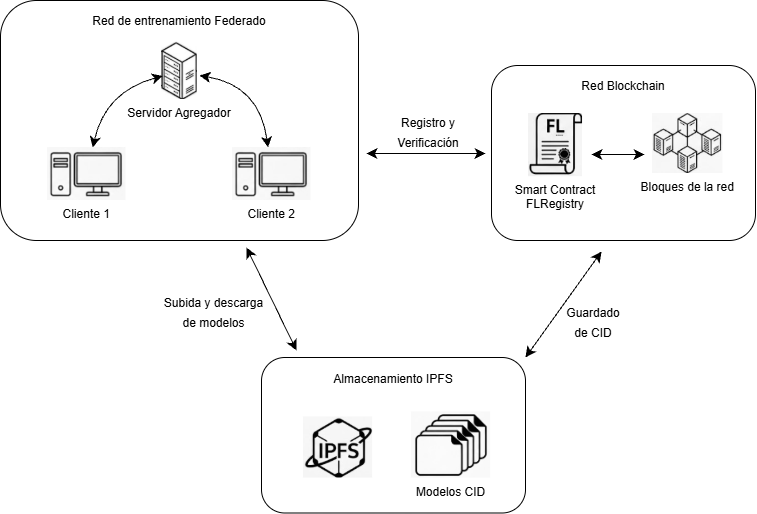
\includegraphics[width=0.88\textwidth]{figuras/ArqSistema.png}
    \caption{Arquitectura general del sistema híbrido: desacoplamiento entre el cómputo federado (Flower), el almacenamiento de pesos fuera de cadena (IPFS) y el registro inmutable de trazabilidad (Hyperledger Besu con IBFT 2.0).}
    \label{fig:arq_sistema}
\end{figure*}

\subsection{Diseño del Smart Contract: FLRegistry}
El componente de gobernanza y auditoría lógica se implementa mediante el contrato inteligente \texttt{FLRegistry}, codificado en Solidity (versión \texttt{0.8.10}). Su misión es registrar un historial criptográfico determinista de cada ronda sin albergar matrices numéricas masivas on-chain.
\\

\subsubsection{Estructuras de datos y persistencia}
La entidad nuclear del contrato es la estructura \texttt{ModelRound}, definida como:
\begin{verbatim}
struct ModelRound {
    uint256 roundNum;
    string modelHash;
    address author;
    uint256 timestamp;
}
\end{verbatim}
donde \texttt{roundNum} indexa la iteración federada, \texttt{modelHash} almacena el CID o digest SHA-256 del artefacto del modelo, \texttt{author} guarda la dirección pública Ethereum del emisor (\texttt{msg.sender}) y \texttt{timestamp} captura la marca temporal del bloque validado.
\\

El estado del contrato se organiza mediante dos tablas hash (\textit{mappings}) complementarias:
\begin{itemize}
    \item \texttt{mapping(uint256 => ModelRound) public \\ history}: almacena de forma secuencial los modelos globales agregados por el servidor al término de cada ronda $t$.
    \item \texttt{mapping(uint256 => mapping(address => \\ ModelRound)) public clientHistory}: indexa las contribuciones locales individuales de cada cliente en cada ronda, posibilitando la auditoría forense granular de las participaciones.
\end{itemize}

Adicionalmente, se mantienen los punteros de estado \texttt{latestRound} y el indicador booleano \texttt{hasModel} para optimizar lecturas directas de acceso constante sin requerir iteraciones sobre el almacenamiento persistente.
\\

\subsubsection{Primitivas de escritura y control de acceso}
El contrato expone dos métodos transaccionales que alteran el estado y emiten el evento desacoplado \texttt{ModelUpdated}:
\begin{itemize}
    \item \texttt{registerClientModel(uint256 round, string memory hash)}: Invocado por cada cliente $k$ tras concluir su entrenamiento local, registrando de forma inmutable el CID de su contribución junto a su dirección Ethereum (\texttt{msg.sender}).
    \item \texttt{updateModel(uint256 round, string memory hash)}: Invocado operacionalmente por el servidor agregador tras converger el algoritmo de agregación. Para salvaguardar la gobernanza de la red y evitar que cualquier participante no autorizado o nodo malicioso pueda registrar modelos globales maliciosos, la función se protege mediante el modificador de control de acceso \texttt{onlyServer}:
    \begin{verbatim}
modifier onlyServer() {
    require(msg.sender == serverAddress, 
            "Emisor no autorizado");
    _;
}
    \end{verbatim}
    donde \texttt{serverAddress} se inicializa en el constructor del contrato con la clave pública del servidor agregador autorizado (pudiendo ser delegada o actualizada mediante esquemas de gobernanza multifirma del consorcio). De este modo, la EVM revierte de manera determinista cualquier invocación no autorizada de \texttt{updateModel}.
\end{itemize}

\subsubsection{Primitivas de lectura y verificación}
Para no sobrecargar la red con costes de ejecución, las consultas de verificación se implementan como funciones \texttt{view}, las cuales se resuelven localmente en el nodo RPC sin consumir gas:
\begin{itemize}
    \item \texttt{getLastModel()}: Permite a cualquier cliente recuperar el CID del último modelo global consolidado y su marca de tiempo.
    \item \texttt{getClientModel(uint256 round, address client)}: Permite al servidor y a auditores externos cotejar el CID reportado por un cliente frente a su registro on-chain firmado.
\end{itemize}

\subsubsection{Generalización y desacoplamiento del modelo}
Conviene destacar que el diseño del marco es conceptual y operativamente agnóstico a la topología de la red neuronal, a la modalidad de los datos y al framework de aprendizaje empleado. Debido a que el contrato \texttt{FLRegistry} gestiona exclusivamente cadenas de longitud uniforme (los CIDs de IPFS y los resúmenes SHA-256), el coste de gas en la EVM permanece predecible y desacoplado de la complejidad del modelo, independientemente de si los parámetros corresponden a un clasificador ligero, una red convolucional profunda o una arquitectura basada en Transformers. Asimismo, el plano de almacenamiento IPFS maneja los pesos serializados como secuencias de bytes genéricas, posibilitando que el protocolo de doble verificación sea extrapolable a diversas modalidades (datos tabulares, series temporales, señales acústicas o visión artificial) y algoritmos de optimización federada.

\subsection{Flujo Operacional y Doble Verificación Cruzada}
El ciclo de vida del entrenamiento federado se estructura en una fase de inicialización única seguida de un protocolo iterativo con verificación bidireccional estricta, como se resume a continuación:
\\

\subsubsection{Fase 0: Arranque y Modelo Base (Ronda 0)}
Antes de iniciar la concurrencia:
\begin{enumerate}
    \item Se inicializa la red Besu con consenso IBFT 2.0 y el daemon IPFS.
    \item Se despliega \texttt{FLRegistry} registrando su dirección y ABI en un descriptor JSON distribuido.
    \item El servidor instancia los pesos iniciales $w^{(0)}$, los serializa y los almacena en IPFS, recibiendo un CID inicial $\text{CID}_0$.
    \item El servidor ejecuta \texttt{updateModel(0, }$\text{CID}_0$\texttt{)}, fijando el punto de partida auditable para todos los participantes. \\
\end{enumerate}

\subsubsection{Fase 1: Verificación Descendente (Cliente protege frente a Servidor)}
Al recibir la señal de inicio de ronda junto con los pesos candidatos $w_{cand}^{(t)}$ vía gRPC (Figura~\ref{fig:flujo_cliente_verif}):
\begin{enumerate}
    \item El cliente consulta la Blockchain invocando \texttt{getLastModel()} y obtiene el $\text{CID}_{reg}^{(t-1)}$ oficial.
    \item El cliente descarga el modelo referenciado desde IPFS y realiza una verificación bit a bit tensor por tensor frente a $w_{cand}^{(t)}$.
    \item Si se detecta cualquier discrepancia entre los pesos entregados y el compromiso sellado en la cadena, el cliente \textbf{aborta el entrenamiento inmediatamente}, neutralizando ataques donde un servidor comprometido intente inyectar modelos sesgados selectivamente a clientes concretos.
\end{enumerate}

\begin{figure}[H]
    \centering
    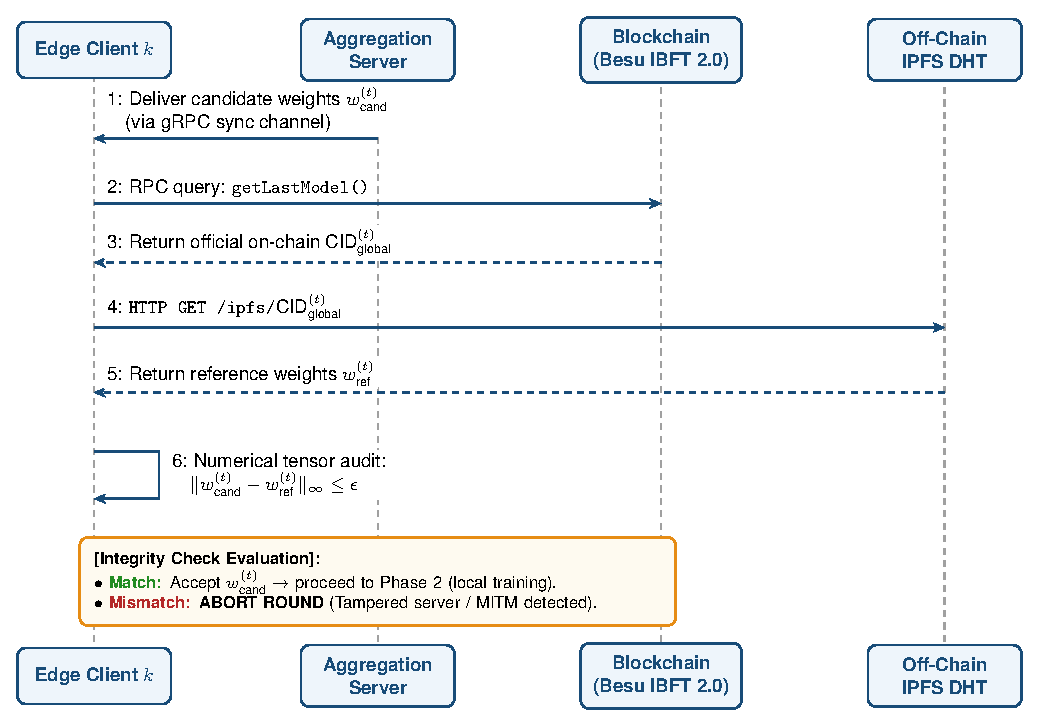
\includegraphics[width=\columnwidth]{figuras/flujo_fase1_verificacion_descendente.pdf}
    \caption{Fase 1: Verificación descendente en el cliente: cotejo del modelo recibido frente al CID registrado on-chain y descargado de IPFS.}
    \label{fig:flujo_cliente_verif}
\end{figure}

\subsubsection{Fase 2: Entrenamiento Local y Registro de Contribución}
Si la comprobación previa es satisfactoria (Figura~\ref{fig:flujo_cliente_entreno}):
\begin{enumerate}
    \item El cliente ejecuta el entrenamiento local con su partición privada de datos.
    \item Serializa los nuevos pesos locales $w_k^{(t)}$ y los almacena en IPFS, obteniendo $\text{CID}_k^{(t)}$.
    \item Emite una transacción firmada con su clave privada invocando \texttt{registerClientModel(}$t$, $\text{CID}_k^{(t)}$\texttt{)} y aguarda el recibo (\textit{receipt}) de inclusión en el bloque IBFT 2.0.
    \item Retorna a Flower los parámetros junto con el identificador $\text{CID}_k^{(t)}$ y su clave pública.
\end{enumerate}

\begin{figure}[H]
    \centering
    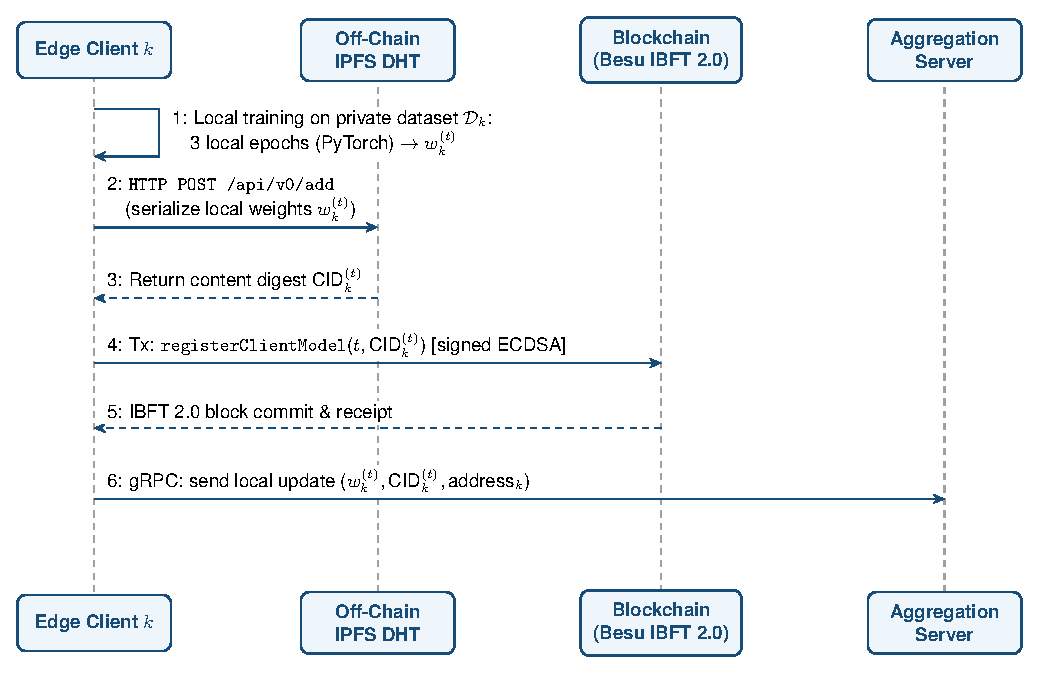
\includegraphics[width=\columnwidth]{figuras/flujo_fase2_entrenamiento_registro.pdf}
    \caption{Fase 2: Entrenamiento local en el cliente, subida de pesos a IPFS y transacción firmada a Hyperledger Besu.}
    \label{fig:flujo_cliente_entreno}
\end{figure}

\subsubsection{Fase 3: Verificación Ascendente y Agregación Global}
Al recibir las actualizaciones de los clientes en el servidor agregador (Figura~\ref{fig:flujo_servidor_agregacion}):
\begin{enumerate}
    \item Para cada cliente $k$, el servidor recibe la carga útil de los parámetros $w_k^{(t)}$ junto con el identificador $\text{CID}_{k,\text{gRPC}}^{(t)}$ y la dirección pública del cliente $\text{address}_k$.
    \item \textbf{Cálculo de integridad local:} El servidor computa de forma determinista el resumen criptográfico del vector de pesos recibido en memoria: $\text{CID}_{k,\text{calc}}^{(t)} = \text{Hash}(w_k^{(t)})$.
    \item \textbf{Consulta on-chain y doble verificación cruzada:} El servidor consulta la función de sólo lectura \texttt{getClientModel($t$, address$_k$)} en \texttt{FLRegistry}, recuperando $\text{CID}_{k,\text{onchain}}^{(t)}$, y valida la condición estricta de doble coincidencia:
    \begin{equation}
    \text{CID}_{k,\text{calc}}^{(t)} == \text{CID}_{k,\text{gRPC}}^{(t)} == \text{CID}_{k,\text{onchain}}^{(t)}
    \end{equation}
    Esta doble comprobación neutraliza dos vectores de ataque complementarios: si un cliente malicioso registrara un CID válido en Besu pero enviara pesos adulterados por gRPC, o si un atacante en red modificara los parámetros en tránsito, $\text{CID}_{k,\text{calc}}^{(t)} \neq \text{CID}_{k,\text{onchain}}^{(t)}$; análogamente, si el CID transmitido por gRPC no se correspondiera con la transacción firmada en Besu, la comprobación fallaría de inmediato. En cualquier caso de discrepancia, la contribución es descartada de forma preventiva antes de la agregación.
    \item Aplica la agregación ponderada FedAvg únicamente sobre las contribuciones debidamente validadas:
    \begin{equation}
    w^{(t+1)} = \sum_{k \in \mathcal{K}_{valid}} \frac{n_k}{n_{valid}} \, w_k^{(t)}
    \end{equation}
    donde $n_k$ representa el número de muestras locales aportadas por el cliente $k$ y $n_{valid} = \sum_{k \in \mathcal{K}_{valid}} n_k$.
    \item Sube el nuevo modelo consolidado a IPFS, obteniendo $\text{CID}_{global}^{(t+1)}$, y lo sella en Besu invocando \texttt{updateModel(}$t+1$, $\text{CID}_{global}^{(t+1)}$\texttt{)}. Dado que \texttt{updateModel} está restringida por el modificador \texttt{onlyServer}, ningún tercero ajeno al agregador designado puede sobrescribir el modelo global.
\end{enumerate}

\begin{figure}[H]
    \centering
    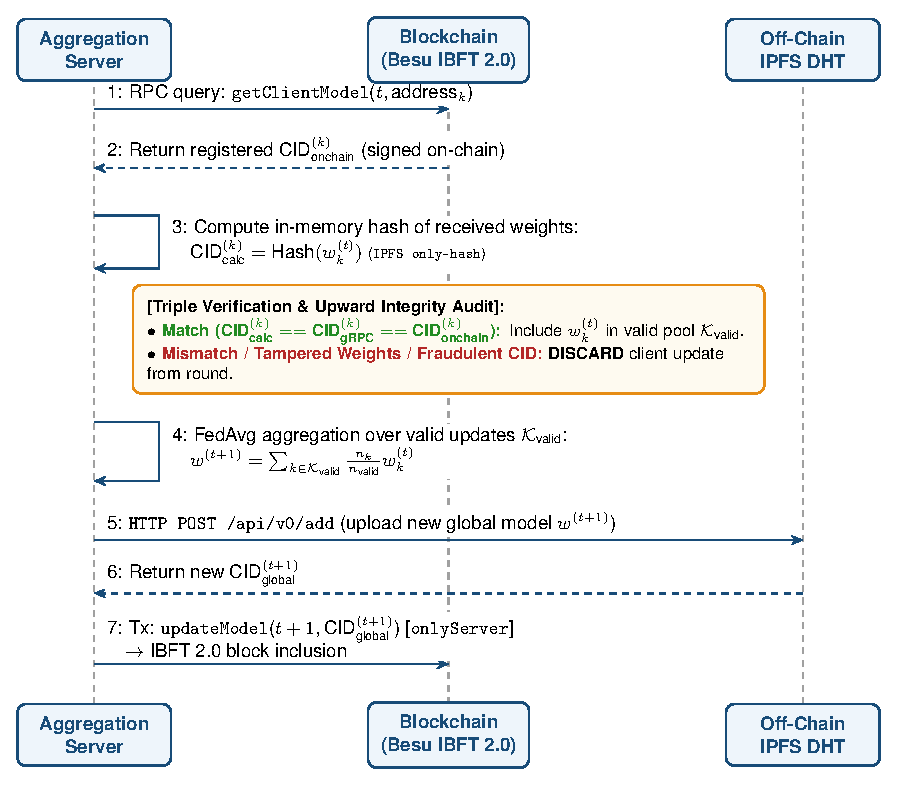
\includegraphics[width=\columnwidth]{figuras/flujo_fase3_verificacion_agregacion.pdf}
    \caption{Fase 3: Verificación ascendente en el servidor: validación de integridad tensorial, verificación on-chain, agregación FedAvg y sellado global de ronda.}
    \label{fig:flujo_servidor_agregacion}
\end{figure}

\subsection{Auditoría Ex-Post y Verificabilidad de FedAvg}
\label{subsec:auditoria_fedavg}
Una propiedad arquitectónica diferencial que se deriva del desacoplamiento híbrido propuesto es la capacidad de verificar de forma determinista y retrospectiva (\textit{ex-post}) el comportamiento del servidor agregador. En los marcos federados convencionales, el servidor actúa como una caja negra de confianza: los clientes deben asumir que los pesos agregados $w^{(t+1)}$ se computaron aplicando honestamente la media ponderada sobre las contribuciones recibidas, sin introducir sesgos no autorizados, omitir clientes arbitrariamente o insertar puertas traseras encubiertas.

En nuestra arquitectura, para cada ronda $t$, quedan registrados de forma inmutable en la cadena de bloques:
\begin{enumerate}
    \item El conjunto de participantes validados $\mathcal{K}_t$ y sus direcciones de cuenta Ethereum.
    \item Los CIDs $\text{CID}_k^{(t)}$ firmados individualmente por cada cliente en \texttt{clientHistory}.
    \item Los volúmenes de datos muestrales $n_k$ correspondientes a cada cliente.
    \item El CID del modelo global resultante $\text{CID}_{global}^{(t+1)}$ registrado por el servidor en \texttt{history}.
\end{enumerate}

Gracias a este registro exhaustivo, cualquier nodo cliente de la federación o una entidad auditora externa independiente puede ejecutar en cualquier instante una verificación determinista de la agregación sin requerir acceso a los conjuntos de datos privados:
\begin{enumerate}
    \item \textbf{Recuperación de artefactos:} El auditor consulta en Besu las direcciones participantes y sus CIDs correspondientes a la ronda $t$, y descarga desde IPFS los vectores de pesos $w_k^{(t)}$.
    \item \textbf{Cotejo de integridad de entrada:} Verifica que para cada cliente $k \in \mathcal{K}_t$, el hash de los pesos descargados coincide con $\text{CID}_k^{(t)}$ sellado en el contrato.
    \item \textbf{Reconstrucción de la agregación:} Aplica formalmente la fórmula determinista de FedAvg:
    \begin{equation}
    \hat{w}^{(t+1)} = \sum_{k \in \mathcal{K}_t} \frac{n_k}{\sum_{j \in \mathcal{K}_t} n_j} \, w_k^{(t)}
    \end{equation}
    \item \textbf{Cotejo del modelo global:} Serializa $\hat{w}^{(t+1)}$ y genera su identificador de contenido $\text{CID}_{audit}^{(t+1)} = \text{Hash}(\hat{w}^{(t+1)})$. A continuación, compara $\text{CID}_{audit}^{(t+1)}$ frente al $\text{CID}_{global}^{(t+1)}$ registrado en \texttt{FLRegistry}.
\end{enumerate}
Si $\text{CID}_{audit}^{(t+1)} \neq \text{CID}_{global}^{(t+1)}$, queda demostrada criptográficamente de manera pública, no repudiable y reproducible la deshonestidad del servidor (ya sea por manipulación de pesos, alteración arbitraria de las ponderaciones $n_k$, o inyección de parámetros maliciosos). Esta verificabilidad transforma la figura del agregador centralizado en un orquestador estrictamente auditable y sujeto a responsabilidad demostrable (\textit{accountability}).

\subsection{Modelo de Amenazas y Alcance de Seguridad}
\label{subsec:modelo_amenazas}
Para delimitar con precisión las garantías provistas por el marco propuesto, se define a continuación el modelo de amenazas considerado, distinguiendo explícitamente entre las vulnerabilidades mitigadas por el diseño arquitectónico y aquellas que quedan formalmente fuera del alcance.

\subsubsection{Amenazas Mitigadas (In-Scope)}
\begin{itemize}
    \item \textbf{Manipulación en tránsito (\textit{Man-in-the-Middle})}: Un adversario en red que intercepte el canal gRPC e intente modificar los tensores locales enviados al servidor o los pesos globales distribuidos a los clientes. Dicha alteración es detectada de forma inmediata gracias al cotejo tensorial bit a bit y a la verificación frente al CID sellado on-chain.
    \item \textbf{Bifurcación y equivocación del servidor (\textit{Server Equivocation / Split-View})}: Un servidor malicioso que intente engañar a clientes específicos enviándoles modelos globales diferentes o adulterados. Dado que los clientes únicamente aceptan pesos cuyo CID coincide unívocamente con el último estado publicado en \texttt{FLRegistry}, cualquier intento de distribución divergente es detectado y bloqueado localmente.
    \item \textbf{Inyección de modelos globales por terceros no autorizados}: Intentos por parte de nodos disidentes o atacantes externos de registrar modelos globales falsos en la Blockchain quedan neutralizados en la EVM mediante el modificador de control de acceso \texttt{onlyServer}.
    \item \textbf{Repudio de contribuciones}: La firma digital basada en criptografía de curva elíptica (ECDSA secp256k1) vinculada a cada transacción en Hyperledger Besu impide que un cliente niegue haber generado o subido una actualización registrada a su nombre.
\end{itemize}

\subsubsection{Amenazas Fuera de Alcance (Out-of-Scope) y Límites del Sistema}
\begin{itemize}
    \item \textbf{Envenenamiento semántico legítimamente firmado (\textit{Semantic Data/Model Poisoning})}: Si un participante genera un modelo malicioso (por ejemplo, mediante técnicas de volteo de etiquetas, \textit{label flipping}, o puertas traseras) a partir de sus propios datos y firma correctamente la transacción en Besu cumpliendo el protocolo, el sistema garantiza la trazabilidad y la atribución no repudiable de la autoría, pero la verificación criptográfica no evalúa la calidad estadística de los gradientes. La defensa ante esta amenaza debe complementarse mediante algoritmos de agregación estadística bizantina robusta (e.g., Krum~\cite{blanchard2017byzantine}, Median o Trimmed Mean) o auditorías forenses posteriores sobre las contribuciones registradas.
    \item \textbf{Compromiso y sustracción de claves privadas (\textit{Key Compromise})}: La validez de las garantías criptográficas descansa sobre la premisa de que las claves privadas de los participantes están debidamente custodiadas. En entornos de producción industrial, este vector exige el empleo de módulos de seguridad de hardware (HSM) o enclaves de ejecución segura (TEE).
    \item \textbf{Ataques de inferencia y reconstrucción de datos crudos (\textit{Inference / Gradient Inversion})}: El protocolo garantiza integridad y procedencia, pero no implementa por defecto mecanismos de Privacidad Diferencial (DP) ni Cómputo Seguro Multipartito (SMPC) sobre los gradientes compartidos.
\end{itemize}

\subsubsection{Privacidad y Exposición de Pesos en IPFS}
En una instancia estándar y pública de IPFS, cualquier participante que conozca el identificador de contenido (CID) podría recuperar los tensores del modelo y potencialmente aplicar técnicas de inferencia para extraer información sobre los datos de entrenamiento locales. Para mitigar esta exposición en entornos consorciados con altos requisitos de confidencialidad (e.g., flotas vehiculares o historiales clínicos), el marco admite dos soluciones de endurecimiento complementarias:
\begin{enumerate}
    \item \textbf{Despliegue de red privada IPFS (\textit{Private Swarm})}: Configuración del daemon IPFS en modo de enjambre privado mediante la definición de una clave compartida (\texttt{swarm.key}) y la variable de entorno \texttt{LIBP2P\_FORCE\_PNET=1}. Esta directiva impide que cualquier nodo ajeno al consorcio se conecte a la red peer-to-peer o resuelva bloques de almacenamiento fuera de los nodos autorizados.
    \item \textbf{Cifrado simétrico en reposo (\textit{Payload Encryption})}: Cifrado de los vectores de parámetros serializados (mediante AES-256-GCM) de forma previa a su subida a IPFS. La clave simétrica de descifrado puede gestionarse mediante esquemas de cifrado híbrido asimétrico dirigidos exclusivamente a las claves públicas de los miembros autorizados del consorcio o esquemas de Cifrado Basado en Atributos (ABE).
\end{enumerate}
